\chapter{Einsatz von KI während der Entwicklung}\label{sec:ki}

Bei der Entwicklung von \textit{helios} kam \textit{GitHub Copilot} in folgenden Bereichen zum Einsatz:

\begin{itemize}
    \itemsep0.5
    \item Vervollständigung von Quellcodekommentaren, insbesondere ortografische und syntaktische Korrekturen.
    \item Erstellung von Dokumentationsblöcken basierend auf den Signaturen von Funktionen, Klassen und Modulen.
    \item Unterstützung bei Compilerfehlern.
    \item Hilfestellung bei der Übertragung von Programmierkonzepten aus anderen Sprachen in C++-idiomatische Konstrukte.
    \item Code Reviews, die auf GitHub beim Erstellen von Pull Requests durchgeführt wurden.
    \item Ausformulieren von Tickets und Anforderungen sowie deren direkte Erstellung als \textit{GitHub Issue}.
    \item Aufsetzen der Projektwebseite~\cite{HeliosProjectHome} unter Anwendung von \textit{docusaurus}~\cite{docusaurus}.
\end{itemize}

Obwohl keine belastbaren Metriken erfasst wurden, haben wir die Nutzung insgesamt als hilfreich wahrgenommen, insbesondere bei Code Reviews.
Ein exemplarisches Beispiel zeigt der in Abbildung~\ref{fig:copilot} dargestellte Kommentar von GitHub Copilot:
Hier weist die KI darauf hin, dass die durch das initiale Hinzufügen der ECS-\textit{Systeme} (siehe Abschnitt~\ref{sec:systems}) hergestellte Ordnung verloren geht, wenn der \textit{View} aufgrund von Änderungen der zu repräsentierenden Datencontainer neu erstellt werden muss.
Konsequenterweise wurde die Umsetzung einem Refactoring unterworfen: Die Lösung wurde über das \textit{Type Erasure}-Idiom  generalisiert.
In einem zusätzlichen Feld wird nun die Einfügereihenfolge festgehalten, um die \textit{View} mit der ursprünglichen Sortierung wiederherzustellen.\\

\begin{figure}[!htbp]
    \centering
    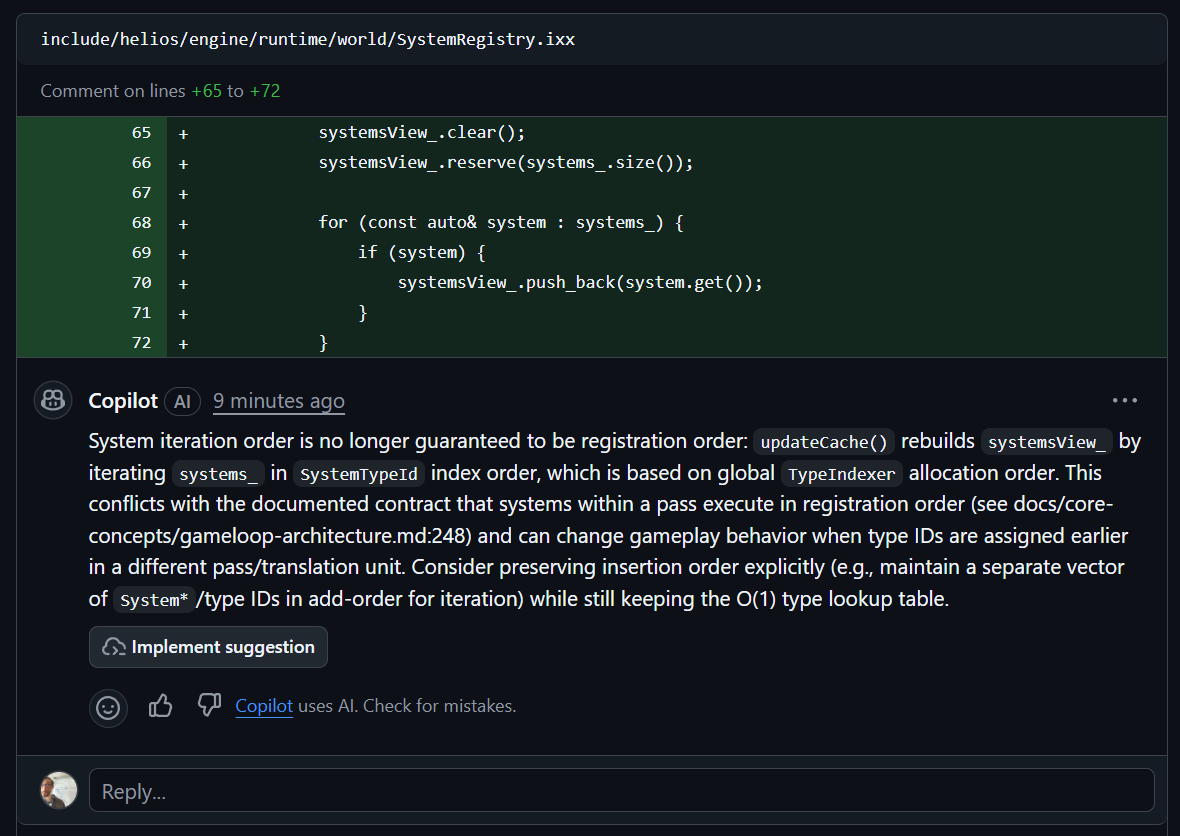
\includegraphics[width=0.8\columnwidth]{content/de/ki/img/copilot}
    \caption{Kommentar von GitHub Copilot in einem Code Review. (Quelle: eigene Aufnahme)}
    \label{fig:copilot}
\end{figure}


In Abbildung~\ref{fig:heliosContributors} ist die Anzahl der Commits von GitHub Copilot im Vergleich zu den Autoren des Projektes dargestellt.

\begin{figure}[!htbp]
    \centering
    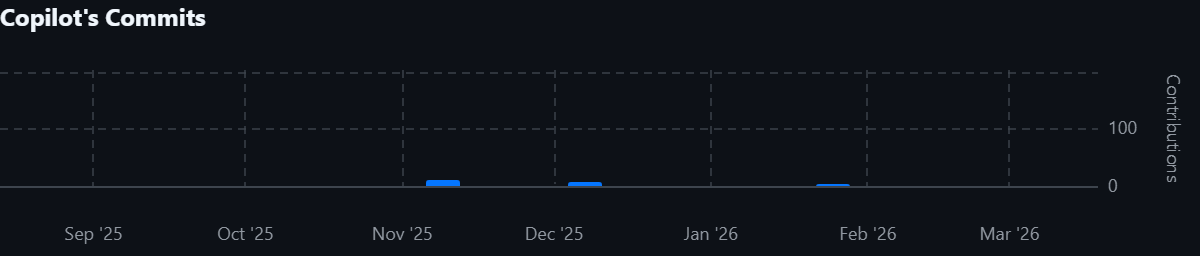
\includegraphics[width=1.0\columnwidth]{content/de/ki/img/Copilot_Commits.png}

    \vspace{0.8em}

    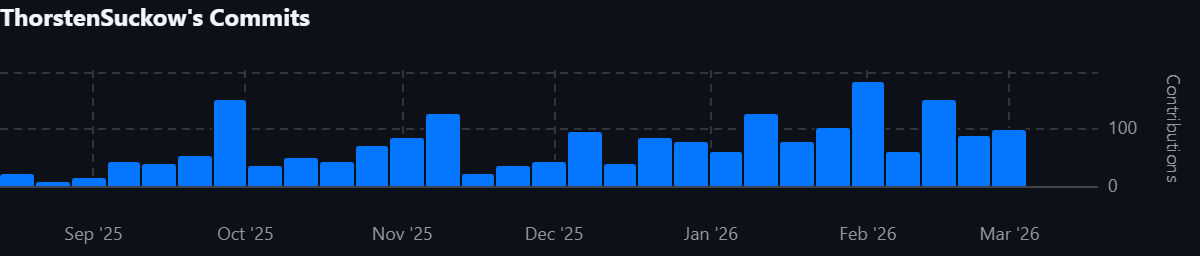
\includegraphics[width=1.0\columnwidth]{content/de/ki/img/ThorstenSuckow_Commits}
    \caption{Vergleich der Commits von GitHub Copilot und den Autoren des Projektes. (Quelle:~\cite{heliosContributors})}
    \label{fig:heliosContributors}
\end{figure}


Während die Anzahl der Commits von Copilot als direkte Beiträge von Anpassungen über die Code-Reviews aufgefasst werden kann, ist die Anzahl der Commits der Autoren nicht direkt mit der Menge des von ihnen geschriebenen Codes korreliert, da einige Commits kleinere Änderungen oder Ergänzungen enthalten, die teilweise von Copilot vorgeschlagen wurden.
So lässt sich der Ausschlag der Commits zum Ende eines jeweiligen Meilensteins nicht bloß auf die Menge von nötigen COde-Anpassungen und Umstrukturierungen der Projektstruktur zurückführen, sondern auch auf die von Copilot angepasste Dokumentation.\\

Insgesamt lässt sich festhalten, dass die durch GitHub Copilot generierten Code Reviews sowie die generierte Dokumentation das Projekt unterstützt haben, auch, wenn die Validierung und Kontextualisierung der Ergebnisse eine zusätzliche Überprüfung bedeutete.


\vspace{5mm}
\begin{tcolorbox}[title={Die Spieleindustrie und der Einsatz von KI}, colback=black!5, colframe=black]
Mit der zunehmenden Verbreitung von KI-gestützten Tools in der Software-Entwicklung, darunter die Integration von Copilot in IDEs wie Visual Studio oder Intellij, steigert sich die Produktivität in der Software Entwicklung zusehends~\cite{githubProductivity}.
Folglich zählt das MIT Technology Review in der Ausgabe 01/2026 \textit {Generative Coding} zu den 10 wichtigsten Technologietrends, und notiert dazu unter anderem, dass - während große Unternehemn wie Microsoft bereits einen Großteil der Codebasis mit Hilfe von KI entwickeln lässt~\cite{heiseAi}, sich gleichzeitig eine Abnahme des Stellenangebots von Junior Positionen abzeichnet.\\

Mit der Welle der Entlassungen großer Studios in den vergangenen Jahren~\cite{gamesindustryLayoffs} sowie der Ankündigung von namhaften Studios, KI in der Spielentwicklung nutzen zu wollen~\cite{larianAi}~\cite{ubisoftAi}, befürchten Konsumenten jedoch um die Qualität der Spiele; gleicherweise Autoren, Grafiken und Synchronsprecher um ihre Arbeitsplätze.~\cite[S. 22]{Soti2026}.
Entsprechend kontrovers wird das Thema in der Spielentwicklung diskutiert.~\cite{pcgameraAi}\\
\end{tcolorbox}
\vspace{5mm}
